%%=============================================================================
%% Methodologie
%%=============================================================================

\chapter{Methodologie}
\label{ch:methodologie}

%% TODO: Hoe ben je te werk gegaan? Verdeel je onderzoek in grote fasen, en
%% licht in elke fase toe welke stappen je gevolgd hebt. Verantwoord waarom je
%% op deze manier te werk gegaan bent. Je moet kunnen aantonen dat je de best
%% mogelijke manier toegepast hebt om een antwoord te vinden op de
%% onderzoeksvraag.

% \lipsum[21-25]

\begin{figure}
	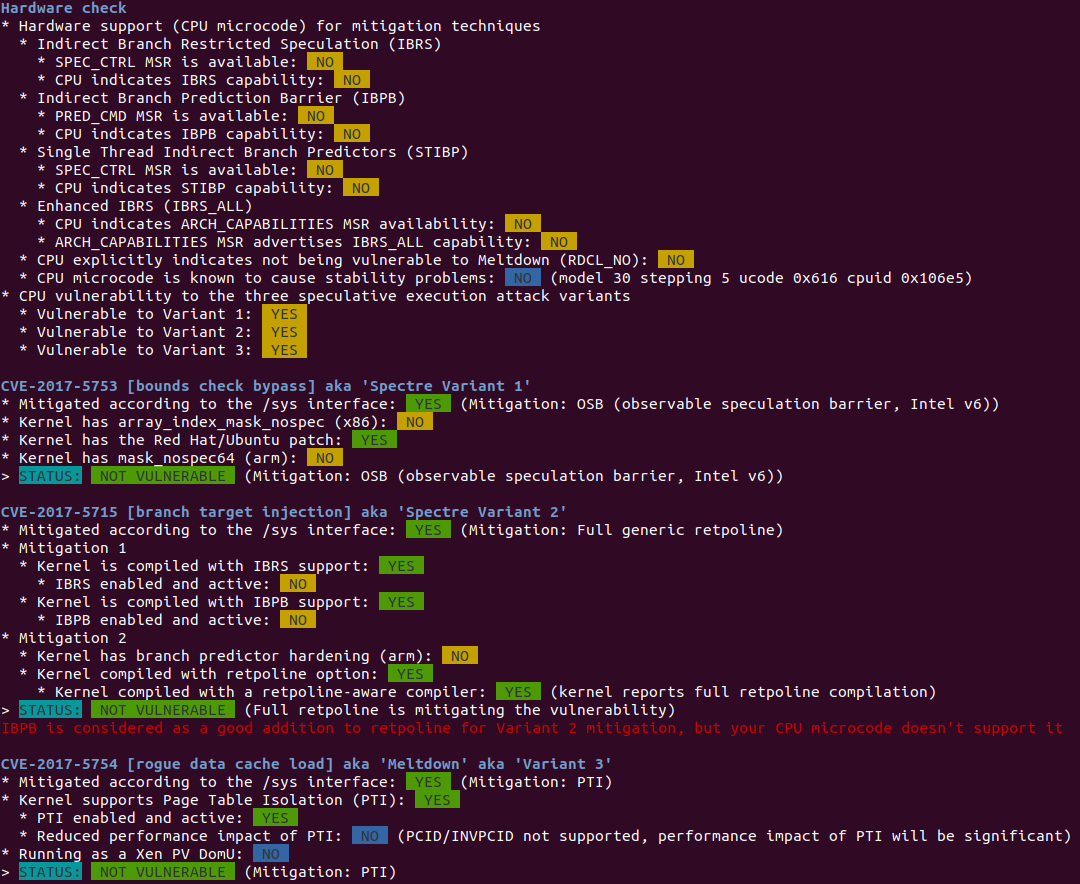
\includegraphics[width=1.0\linewidth]{img/checker_patched.png}
	\caption{Kwetsbaarheid checker beveiligd systeem}
	\label{fig:checker_patched}
\end{figure}

\begin{figure}
	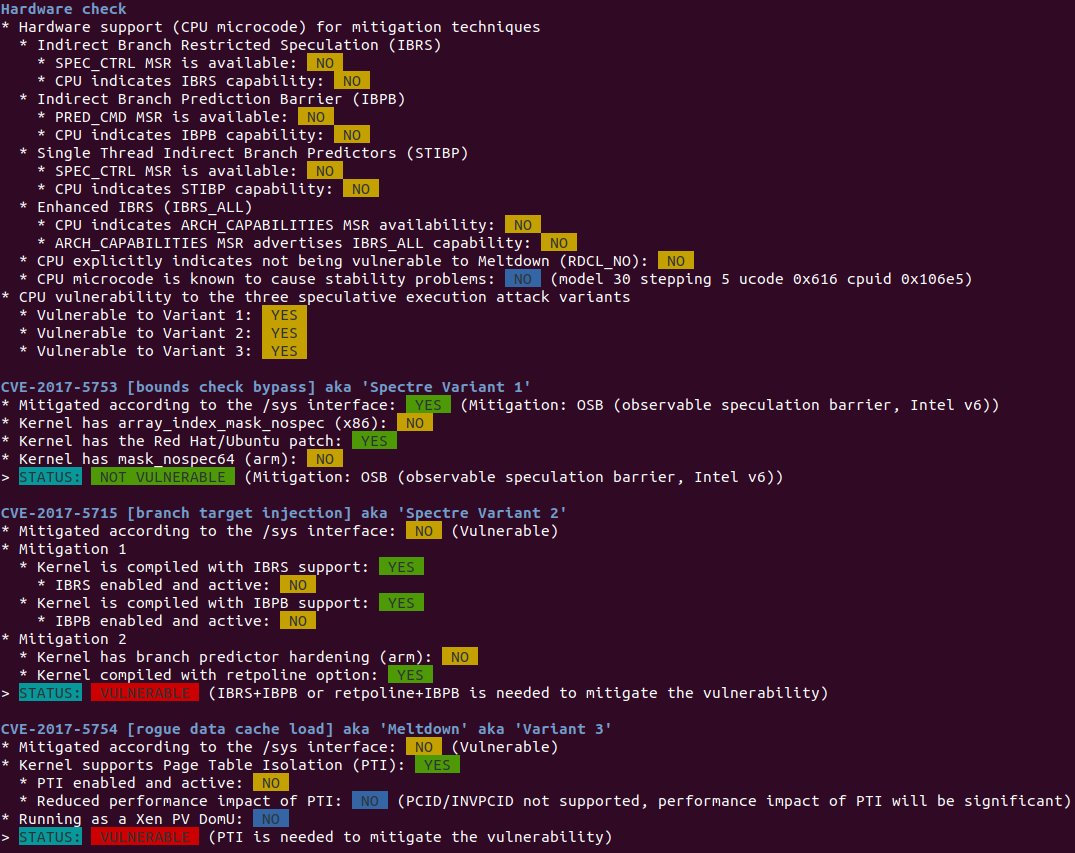
\includegraphics[width=1.0\linewidth]{img/checker_vulnerable.png}
	\caption{Kwetsbaarheid checker kwetsbaar systeem}
	\label{fig:checker_vulnerable}
\end{figure}

Voor de uitwerking van deze scriptie werd eerst de testopstelling opgezet.\\
Dit is gedaan met behulp van Vagrant.\\
Er werd gekozen voor Vagrant omdat dit een snelle en reproduceerbare manier is om meerdere virtuele machines op te zetten. Om de servers te configureren werd Ansible gebruikt.

\section{Opstelling}
De volledige setup is gedefinieerd in één file: de Vagrantfile.
In de Vagrantfile zijn er drie virtuele machines gedefinieerd. Twee ervan zijn webservers: één kwetsbaar voor meltdown en spectre, en één met de patches. De andere is een client die de belasting genereert. Het besturingssysteem is Ubuntu 14.04 64-bits. Dit besturingssyteem zit in de trusty64 vagrant box. Er werdt gekozen voor deze box omdat het regelmatig geüpdate wordt en door Canonical zelf wordt onderhouden.\\
De virtuele machine provider is virtualbox. Provisioning wordt voorzien door ansible en is in vagrant geconfigureerd.

\section{Patches}
Standaard zijn de patches geïnstalleerd, het is dus een kwestie van ze uit te schakelen voor de kwetsbare server.
Dit wordt gedaan via kernel parameters. Er worden items toegevoegd aan het einde van de 'grub kernel' opdrachtregel voor zowel normale als herstelmodi.
Alleen de patches voor variant 2 en variant 3 (meltdown) zijn uitgeschakeld (figuur \ref{fig:checker_patched} en \ref{fig:checker_vulnerable}) omdat variant 1 geen meetbare impact heeft \parencite{Redhat2018a}.